\section{Typage}

\subsection{Typage naïf et génération des contraintes}

\subsubsection{Implémentation de \texttt{type\_of\_built\_in} et \texttt{type\_expr}}

Commençons par implementer \texttt{type\_of\_built\_in}. Elle associe un type à chaque opération built\_in du langage.
Application des vérifications de type built\_in commentées dans \texttt{ast.mli}.

Ensuite, la fonction \texttt{type\_expr} a pour rôle d'inférer le type d'une expression du langage source, tout en produisant un ensemble de contraintes de typage.
Ces contraintes seront résolues ultérieurement lors de la phase d'unification.

\texttt{type\_expr} procède par analyse structurelle de l'expression en entrée. Pour chaque forme syntaxique, elle infère un type approprié et génère si nécessaire des contraintes de typage. 
Les constantes entières, booléennes ou chaînes sont directement typées en \texttt{TInt}, \texttt{TBool} ou \texttt{TString}, sans contrainte. Les fonctions primitives sont, quant à elles, typées à l'aide de la fonction \texttt{type\_of\_built\_in}, qui peut retourner des types monomorphes ou polymorphes. 
L'expression \texttt{Nil}, représentant la liste vide, est typée comme une liste contenant un type inconnu \texttt{TList([], a)}. Les expressions unitaires sont simplement typées en \texttt{TUnit}. 

Lorsqu'une variable est rencontrée, son type est récupéré dans l'environnement, une absence déclenche une erreur. Les abstractions de fonctions (\texttt{Fun}) sont typées en générant un type inconnu pour l'argument, puis en inférant le type du corps avec ce nouvel argument dans l’environnement, on construit alors le type de fonction \texttt{TFunc([], arg\_ty, ret\_ty)}.
L'application de fonction (\texttt{App}) introduit une contrainte cruciale : le type de la fonction doit correspondre à une application du type de l'argument vers un type résultat encore inconnu.
Cette relation est capturée par une contrainte entre le type de l'expression fonctionnelle et un type \texttt{TFunc([], arg\_ty, res\_ty)}.

L'expression conditionnelle (\texttt{IfThenElse}) impose deux contraintes : la condition doit être de type booléen, et les deux branches doivent être de même type.
Pour l'expression séquentielle (\texttt{Ignore}), seul le type de la seconde sous-expression est conservé, tandis que les contraintes des deux expressions sont agrégées.
Enfin, dans les expressions \texttt{Let}, une variable est liée à une expression. Si la déclaration est récursive, une variable de type est d'abord insérée dans l'environnement avant l'inférence de \texttt{e1}, puis une contrainte d'égalité est ajoutée entre cette variable et le type effectivement trouvé.
Ensuite, la variable est de nouveau ajoutée à l'environnement pour inférer le type de \texttt{e2}, qui sera celui de l'expression globale.

Ainsi, chaque forme syntaxique correspond à un schéma de typage local, et les contraintes collectées permettront, dans une étape ultérieure, de résoudre les incertitudes via un algorithme d'unification.

\subsubsection{Exemples programmes mini-ml}
Nous donnons 3 exemples de code mini-ml pour tester notre type\_expr :

Le premier, \texttt{simple1.mml}, ne fait rien et renvoie la valeur transmise.

\begin{lstlisting}
let nothing n =
    (* annot n : 'b *)
        n
        (* nothing 'b -> 'b *)
    
    let main =
        nothing 5
    \end{lstlisting}

Le second, \texttt{simple2.mml} renvoie "prince ali" si la paramètre reçu est vrai, sinon il renvoie "prince arda" qui n'est pas le prince Ali.

\begin{lstlisting}
let prince = fun b ->
(* annot b :'b *)
        if b = true then
            "ali"
        else
            "arda"
        (* prince : 'b -> string *)
    let main =
      prince true
        \end{lstlisting}

Le troisième, \texttt{simple3.mml}, renvoie l'effort total realisé pour le projet Mini-ml, si un paramètre a fait plus de travail que l'autre, il est incrémenté.

\begin{lstlisting}
let rec project a b =
(* annot a : 'b, b : 'c *)
    if a < b then
        project (a + 1) b
        (* contraints :
        ('b, TInt) pour a < b
        ('c, TInt) pour a + 1
        retour project : 'i = result type universel fresh *)
    else if b > a then
        project a (b + 1)
        (* contraints analogues pour b > a et b+1 *)
    else
        a + b
        (* contraints ('b = TInt), ('c = TInt) et result TInt *)
        (* project : 'b -> 'c -> 'i *)
let main =
  project 4 6
            \end{lstlisting}

Nous choisissons le programme \texttt{prince} pour illustrer pas à pas le fonctionnement de notre typeur naïf :

La figure \ref{fig:TypageEx2Graph} donne l’arbre AST annoté avec les types :

\begin{figure}[!ht]
    \centering
    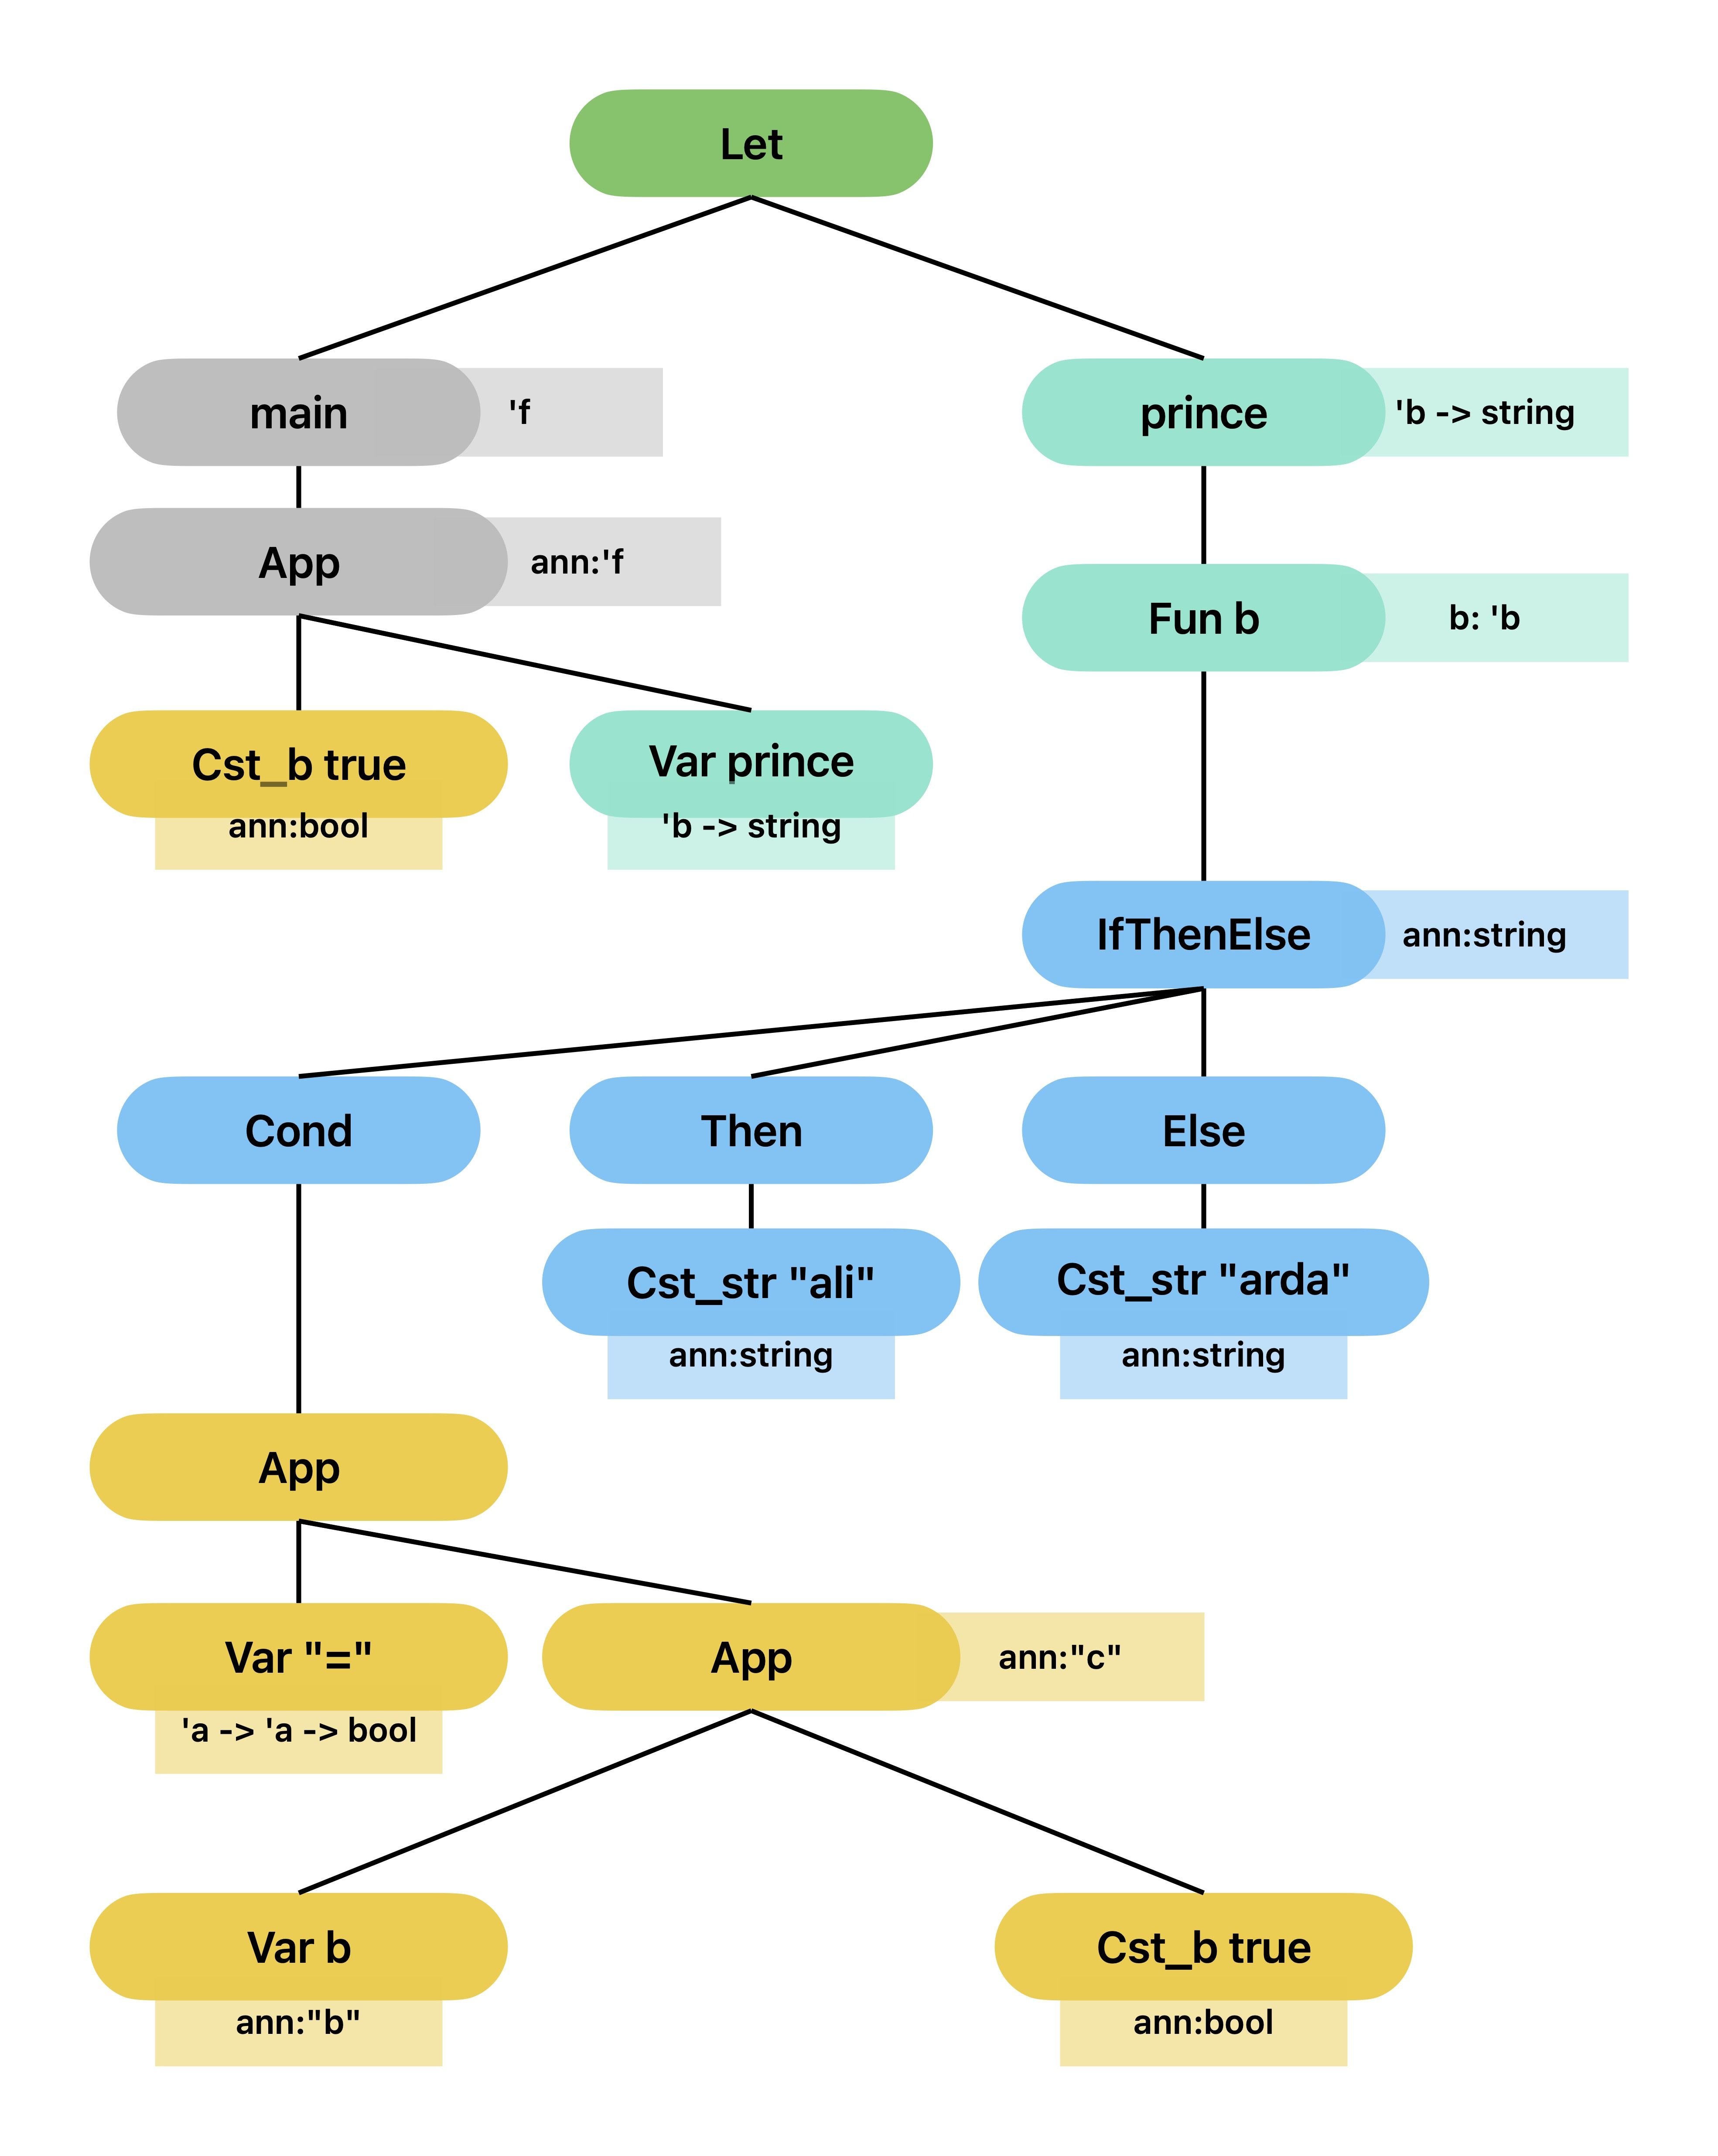
\includegraphics[width=0.7\textwidth]{images/TypageEx2Graph.jpg}
    \caption{Arbre AST annoté pour \texttt{simple2.mml}, avec types}
    \label{fig:TypageEx2Graph}
\end{figure}

\begin{itemize}
    \item \textbf{Paramètre \texttt{b}}, b : 'b (aucune contrainte à ce stade)

    \item \textbf{Appel de \(\texttt{=}\)} sur \(\texttt{b = true}\) :
          \[
              (\,'a \to 'a \to \mathsf{bool}\,) = ('b \to 'c)
              \;\Longrightarrow\;
              \boxed{('a \to 'a \to \mathsf{bool}) = ('b \to 'c)}
          \]
          puis le résultat de \(\texttt{=}\) est un \(\mathsf{bool}\), donc
          \[
              'c = (\mathsf{bool} \to 'd),
              \quad
              'd = \mathsf{bool}.
          \]

    \item \textbf{Branche \texttt{then}}, "ali" : string (pas de contrainte)

    \item \textbf{Branche \texttt{else}}, "arda" : string contrainte triviale : string = string.

    \item \textbf{IfThenElse} :
          l’ensemble des contraintes recueillies ici est
          \[
              \{ ('b = \mathsf{bool}),\;('c = \mathsf{bool}\to 'd),\;('d = \mathsf{bool}),\;(\mathsf{string} = \mathsf{string})\}.
          \]
          Le type final de la condition est alors \(\mathsf{string}\).

    \item \textbf{Définition de \texttt{prince}}, prince : 'b -> string.

    \item \textbf{Appel \(\texttt{prince true}\)} :
          on unifie
          \[
              ('b \to \mathsf{string}) = (\mathsf{bool} \to 'f)
              \;\Longrightarrow\;
              'b = \mathsf{bool},\; 'f = \mathsf{string}.
          \]

    \item \textbf{Définition de \texttt{main}} : 'f, 'f = string.
\end{itemize}

Après unification complète, on obtient :
\[
    prince : \mathsf{bool} \to \mathsf{string},
    \quad
    main   : \mathsf{string}.
\]

\paragraph{}
On constate que les deux jeux de contraintes diffèrent uniquement par le nommage et le regroupement des variables universelles, et non par leur structure. Dans la version correcte, on écrit explicitement
\[
    ('a \to 'a \to \mathsf{bool} = 'c \to 'd),\;('c = 'b),\;('d = 'e \to 'f),\;('e = \mathsf{bool}),\;('f = \mathsf{bool})
\]
tandis que dans notre version, nous avons simplement renommé et fusionné certains équations pour obtenir
\[
    ('a \to 'a \to \mathsf{bool} = 'b \to 'c),\;('c = \mathsf{bool} \to 'd),\;('d = \mathsf{bool}).
\]
Un raisonnement analogue vaut pour les contraintes associées à \texttt{main}. Après unification, les deux approches donnent le même résultat :
\[
    prince : \mathsf{bool} \to \mathsf{string}
    \quad\text{et}\quad
    main : \mathsf{string}.
\]
Ainsi, nos contraintes sont et produisent la même instanciation finale, ce qui montre que notre typage faible est correct.

\subsection{Résolution des contraintes et polymorphisme faible}

Après avoir implémenté \texttt{solve\_constraints}, notre typeur devrait être capable de détecter si le programme analysé est correct.
Essayons-le sur les trois exemples :

\begin{lstlisting}
--Weak typing Example 1--
  nothing : 'b -> 'b 
    constraints : []
  main : 'd 
    constraints : [,'b -> 'b = int -> 'd]
---Solving constraints:
  nothing : 'b -> 'b
  main : int
  Annotated program:
  let nothing (n : 'b) : 'b =
    (n : 'b)
  let main : int =
    (nothing : int -> int) 5

--Weak typing Example 2--
    prince : 'b -> string 
      constraints : [,(,'a)'a -> ...,string = string]
    main : 'f 
      constraints : [,'b -> string = bool -> 'f]
---Solving constraints:
    prince : bool -> string
    main : string
    Annotated program:
    let prince (b : bool) : string =
      if (b : bool) = true then
        "ali"
      else
        "arda"
    let main : string =
      (prince : bool -> string) true
    
--Weak typing Example 3--
      project : 'b -> 'c -> 'i 
        constraints : [,'a = 'b -> 'c -> 'i,...,'i = 'o]
      main : 't 
        constraints : [,'b -> 'c -> 'i = int -> 's,'s = int -> 't]
---Solving constraints:
      project : int -> int -> int
      main : int
      Annotated program:
      let rec project (a : int) (b : int) : int =
        if (a : int) < (b : int) then
          (project : int -> int -> int) ((a : int) + 1) (b : int)
        else
          if (b : int) > (a : int) then
            (project : int -> int -> int) (a : int) ((b : int) + 1)
          else
            (a : int) + (b : int)
      let main : int =
        (project : int -> int -> int) 4 6
\end{lstlisting}

Ces trois exemples semblent syntaxiquement corrects.

Donc pour tester, nous allons l'exécuter sur un exemple incorrect dans

\texttt{/examples/incorrect/extended\_syntax/add\_bool\_int.mml} :

\begin{lstlisting}
--Weak typing--
  x : 'c 
    constraints : [,int -> int -> int = int -> 'b,'b = bool -> 'c]
---Solving constraints:
  Unable to unify int and bool
  Annotated program:
  let x : 'c =
    4 + true
\end{lstlisting}

Cela nous montre qu'il n'est pas capable d'ajouter un entier à un booléen ce qui est normal.

Pour le programme au debut du chapitre:
\begin{lstlisting}
let f = fun x -> x
let a = f 1
let b = f "coucou"
\end{lstlisting}

Nous constatons l'erreur suivante: Unable to unify int and string.
La définition let \texttt{f = fun x -> x} se voit d’abord attribuer un type monomorphe \texttt{'b -> 'b}, puis l'appel f 1 unifie 'b avec int (donnant a : int), mais le second qui appel f "coucou" cherche à réunifier 'b avec string, ce qui échoue (int != string) dans un système à polymorphisme faible.

Parallèlement à cet exemple, nous pouvons en donner un autre qui n'est pas correctement typé alors que OCaml le
type, typer1.mml:

\begin{lstlisting}
let choisir = fun x -> fun y -> x
let a = choisir 1 2
let b = choisir "hokus" "pokus"
\end{lstlisting}

L'appel \texttt{choisir 1 2} impose 'b = int et 'c = int pour que le résultat soit \texttt{int}, ce qui fixe la fonction \texttt{choisir} à \texttt{int -> int -> int} et donne \texttt{a : int}.
Ensuite, le second appel choisir \texttt{"hokus" "pokus"} tente d'unifier avec \texttt{string -> \_ -> string}, mais comme 'b est déjà fixé à int, la contrainte \texttt{int = string} échoue et génère l'erreur d'unification.

\subsection{Typage fortement polymorphe}

\subsubsection{\texttt{instantiate}}

La fonction \texttt{instantiate} permet de gérer le polymorphisme fort en remplaçant les variables de type quantifiées dans un type polymorphe par des variables de type universelles fraîches. 
Elle est essentielle dans l'algorithme de typage pour assurer que chaque utilisation d'un terme polymorphe se fasse avec des variables de type distinctes, évitant ainsi toute confusion lors de la résolution de contraintes.

Elle prend en paramètre :
\begin{itemize}
  \item \texttt{counter} : un compteur de variables universelles, utilisé pour générer des indices frais (\texttt{TUniv n})
  \item \texttt{type\_lang} : un type potentiellement polymorphe contenant une liste de types génériques à instancier
\end{itemize}

\textbf{Principe de fonctionnement} :
\begin{enumerate}
  \item Si le type est polymorphe (\texttt{TFunc} ou \texttt{TList} avec une liste \texttt{generics} non vide), on associe chaque identifiant de type générique à un nouvel identifiant frais, généré par le compteur
  \item On crée une substitution (liste d’associations) de ces anciens identifiants vers les nouveaux
  \item On applique récursivement cette substitution à l'ensemble des sous-types du type initial (type d'argument, type de retour ou type d'éléments)
  \item On retourne un nouveau type identique, sauf que la liste des \texttt{generics} est vidée (le type est monomorphe)
\end{enumerate}

Cette instanciation est indispensable à chaque appel de fonction dans le typeur afin de garantir que les variables de type restent indépendantes entre chaque appel.

\subsubsection{Version finale de \texttt{type\_expr}}

La fonction \texttt{type\_expr} constitue le cœur de l'inférence de types dans notre langage. Dans sa version finale, elle est capable de prendre en charge le polymorphisme fort, notamment dans le cadre des expressions \texttt{let} et des appels de fonction \texttt{App}.
La première version de \texttt{type\_expr} proposait une approche naïve, où toutes les contraintes étaient collectées globalement, puis résolues en une seule étape à la fin. Cela suffisait pour un typage monomorphe, mais ne permettait pas de gérer correctement le polymorphisme.

Dans la version finale, les principales modifications sont les suivantes :
\begin{itemize}
  \item \textbf{Résolution locale des contraintes} dans les expressions \texttt{let} : les contraintes internes à l'expression \texttt{e1} de \texttt{let x = e1 in e2} sont résolues immédiatement. On applique ensuite la substitution obtenue à \texttt{e1} et à l'environnement avant de généraliser son type
  \item \textbf{Généralisation explicite} du type de \texttt{e1} après résolution locale : les variables universelles qui n’apparaissent pas dans l’environnement sont marquées comme génériques
  \item \textbf{Instanciation des types} dans les applications de fonction \texttt{App(f, arg)} : on remplace les types génériques par des variables fraîches via la fonction \texttt{instantiate}
  \item \textbf{Propagation des contraintes} : les contraintes issues des sous-expressions sont concaténées, et des contraintes supplémentaires (comme la compatibilité fonctionnelle) sont ajoutées localement
\end{itemize}

La signature \texttt{type\_lang * (type\_lang * type\_lang) list} est essentielle pour plusieurs raisons :
\begin{itemize}
  \item permet de différer la résolution des contraintes jusqu'à ce qu'elles soient suffisamment isolées (par exemple dans un \texttt{let})
  \item autorise une approche modulaire et incrémentale du typage, chaque nœud syntaxique pouvant générer ses propres contraintes
  \item s’intègre parfaitement avec le mécanisme de résolution \texttt{solve\_constraints}, qui prend en charge la substitution des types et la détection d'erreurs de typage
\end{itemize}

En résumé, cette nouvelle version de \texttt{type\_expr} respecte les règles du polymorphisme fort tout en restant modulaire, et sa signature permet de gérer proprement les contraintes générées par chaque expression.

\subsubsection{Exemple de typage avec polymorphisme fort}

Considérons l'exemple décrit en début de section. Grâce à l'introduction du polymorphisme fort, cette séquence d'expressions est bien typée. 
Lors du typage de \texttt{let f = fun x -> x}, une variable de type universelle $TUniv(0)$ est attribuée à \texttt{x}, et le corps de la fonction \texttt{x} est du même type. 
Le type obtenu est donc $TFunc([], TUniv(0), TUniv(0))$, qui est ensuite généralisé par rapport à l'environnement, produisant le type polymorphe $TFunc([0], TUniv(0), TUniv(0))$. 
Lors de l'appel \texttt{f 1}, ce type est instancié avec une nouvelle variable universelle, par exemple $TUniv(1)$, qui est ensuite contrainte à être égale à \texttt{TInt}. 
On obtient donc que \texttt{a} est de type \texttt{int}. De même, dans l'appel \texttt{f " coucou "}, une nouvelle instanciation du type de \texttt{f} permet de typer l'expression avec $TString$, ce qui donne \texttt{b : string}. 
Cet exemple illustre que le polymorphisme fort permet à une même fonction générique d’être utilisée avec des types différents sans redéfinition, en généralisant son type à la déclaration, puis en l'instanciant à chaque utilisation.

\subsubsection{Comparaison entre typage naïf et polymorphisme fort}

Considérons les deux exemples suivants, qui illustrent des situations où le typage polymorphe offre plus de flexibilité que le typage naïf.

\begin{lstlisting}
let id = fun x -> x
let a = id true
let b = id 42
\end{lstlisting}

Dans ce premier exemple, la fonction \texttt{id} est générique. Avec un typeur naïf, le premier appel à \texttt{id} fixe son type (ici \texttt{bool -> bool}), ce qui empêche la réutilisation avec un autre type (ici \texttt{int}).
Avec le polymorphisme fort, \texttt{id} est généralisée en \texttt{forall 'a. 'a -> 'a}, rendant son typage indépendant pour chaque appel.

Le second exemple met en évidence le même phénomène dans un contexte de fonctions plus riches :

\begin{lstlisting}
let add = fun x -> fun y -> x + y
let id = fun z -> z
let _ = id (add 1)
let _ = id (fun s -> s ^ "!")
\end{lstlisting}

Sous le typeur naïf, la fonction \texttt{id} est typée lors du premier appel avec \texttt{add 1}, ce qui lui donne le type \texttt{int -> int}.
Le second appel avec une fonction sur les chaînes de caractères échoue, car \texttt{id} ne peut plus être typée avec \texttt{string -> string}.
Le typeur avec polymorphisme fort, quant à lui, généralise \texttt{id}, et autorise ces deux appels indépendamment grâce à l'instanciation du type générique.
C'est une démonstration claire de la puissance du polymorphisme fort dans la réutilisation sécurisée et typée de fonctions génériques.